% TODO[HLA-FIX 2026-06-27]: PredIG 全局显著性已失效(max-pool rho 0.198->0.104 p=0.343 ns; mean-agg 0.280->0.188 p=0.084 ns)，剔污染患者 P101/P102 后不存活；IMPROVE 仍稳健显著(0.226 p=0.037)，TSCAPE 翻为显著负(-0.230 p=0.033)，deepHLApan 另有 merge bug 双重不可信；per-patient 头条数字(PRIME/deepHLApan)待 Phase B 正确等位重推理后更新。正文数字暂不动(投稿=拍板点 + P102 等位待袁老师确认)。详见 04_LOG Entry HLA-FIX。
\section{Results}
\label{sec:results}

We organize the results around the two empirical claims of the paper. First, no
tool in the panel recovers the \emph{magnitude} of the T-cell response with more
than weak correlation, and the binary discrimination ranking, while it has a
clear point-estimate leader, is not statistically separable and is sensitive to
the aggregation and threshold conventions (Sections~\ref{sec:res-global}
and~\ref{sec:res-sensitivity}). Second, moving from a single pooled
(``global'') correlation to a per-patient protocol reorders the panel and
surfaces individual-level structure that the global metric conceals
(Section~\ref{sec:res-perpatient}). The presentation proxy serves throughout as a
near-random calibration anchor (Section~\ref{sec:res-proxy}). Unless stated
otherwise, all numbers use the locked primary configuration: best-binder
(maximum) aggregation and the SFC $>0$ threshold on DS2.

\subsection{Global head-to-head comparison}
\label{sec:res-global}

Table~\ref{tab:main} reports the primary apples-to-apples comparison of the eight
immunogenicity predictors under the locked configuration. Two patterns are
immediate. First, the continuous-magnitude signal is weak across the board: every
tool has $|\rho| < 0.33$ for the Spearman correlation between its score and the
ELISpot SFC value, and only two tools reach nominal significance at this
operating point---IMPROVE ($\rho = 0.2434$, $p = 0.0142$) and PredIG
($\rho = 0.1983$, $p = 0.0468$). The remaining six tools have correlations that
are not significantly different from zero, with NeoTImmuML$^\star$
($\rho = 0.0218$, $p = 0.8285$) and deepHLApan ($\rho = 0.0415$, $p = 0.6847$)
effectively at the noise floor and DeepImmuno carrying a small negative point
estimate ($\rho = -0.1168$, $p = 0.2449$). In other words, even the two
significant correlations explain only a few percent of the rank variance in
response magnitude, and no tool in the panel supports a quantitative regression of
ELISpot SFC. These two nominal significances are moreover uncorrected for the
eight tools tested; under a Bonferroni correction at $\alpha = 0.05$ (threshold
$p < 0.00625$) neither survives, which only strengthens the conclusion that the
panel as a whole does not recover magnitude.

Second, binary discrimination has a clear point-estimate ordering but a narrow
spread in practical terms. pTuneos attains the highest AUC-ROC point estimate
($0.7525$), followed by PredIG ($0.6611$) and NeoTImmuML$^\star$ ($0.6551$); the
lower half of the panel sits near or below chance, with DeepImmuno ($0.4813$) and
deepHLApan ($0.4188$) falling under $0.5$ at this operating point. We caution
against reading this column as a definitive ranking: as Section~\ref{sec:res-sensitivity}
shows, the leading AUC is both statistically indistinguishable from its nearest
competitors and sensitive to the aggregation and threshold choice. The AUPRC
values are uniformly high ($0.895$--$0.949$) but offer limited headroom, because
the positive class makes up roughly $89\%$ of the cohort and the no-skill AUPRC
baseline is already $\approx 0.891$; the AUPRC differences across tools are
therefore small relative to this baseline and should not be over-interpreted.

\begin{table}[t]
\centering
\caption{Primary head-to-head comparison on DS2 under the locked configuration
(best-binder aggregation, SFC $>0$ threshold; $n = 101$ peptides unless noted).
AUC-ROC and AUPRC measure binary discrimination; Spearman $\rho$ (with $p$-value)
measures recovery of continuous response magnitude. The no-skill AUPRC baseline at
this threshold is $\approx 0.891$ ($90/101$ positive). Tools are ordered by
AUC-ROC point estimate; this ordering is \emph{not} statistically separable
(Section~\ref{sec:res-sensitivity}, Table~\ref{tab:bootstrap}).
NeoTImmuML$^\star$ denotes the self-retrained model (official weights
unavailable). Effective sample size is reduced for PRIME ($n = 100$) and
deepHLApan ($n = 98$); see Table~\ref{tab:coverage}.}
\label{tab:main}
\begin{tabular}{lcccc}
\toprule
Tool & AUC-ROC & AUPRC & Spearman $\rho$ & $p$ \\
\midrule
pTuneos            & $0.7525$ & $0.9494$ & $0.1363$  & $0.1741$ \\
PredIG             & $0.6611$ & $0.9411$ & $0.1983$  & $0.0468^{*}$ \\
NeoTImmuML$^\star$ & $0.6551$ & $0.9421$ & $0.0218$  & $0.8285$ \\
IMPROVE            & $0.6207$ & $0.9221$ & $0.2434$  & $0.0142^{*}$ \\
ImmuneApp          & $0.5889$ & $0.9080$ & $0.0885$  & $0.3786$ \\
PRIME$^{\,n=100}$  & $0.5276$ & $0.9146$ & $0.1163$  & $0.2491$ \\
DeepImmuno         & $0.4813$ & $0.8951$ & $-0.1168$ & $0.2449$ \\
deepHLApan$^{\,n=98}$ & $0.4188$ & $0.9038$ & $0.0415$ & $0.6847$ \\
\bottomrule
\end{tabular}

\vspace{2pt}
{\footnotesize $^{*}$ $p < 0.05$. The two significant correlations
(IMPROVE, PredIG) nonetheless correspond to $|\rho| \le 0.25$.}
\end{table}

\begin{figure}[t]
\centering
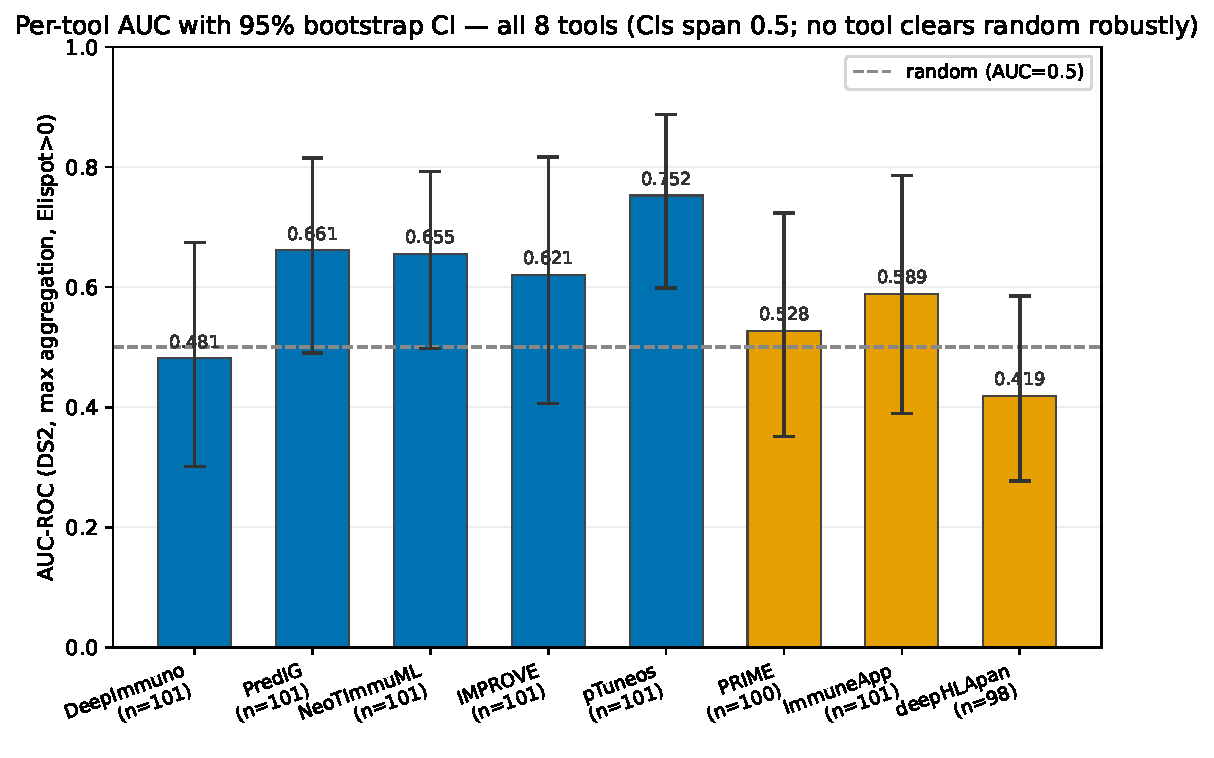
\includegraphics[width=\linewidth]{figures/fig6_auc_comparison.pdf}
\caption{AUC-ROC for the eight tools at the three thresholds (SFC $>0$, $>10$,
$>$ median) under best-binder aggregation. New-wave tools are highlighted.}
\label{fig:auc}
\end{figure}

\begin{figure}[t]
\centering
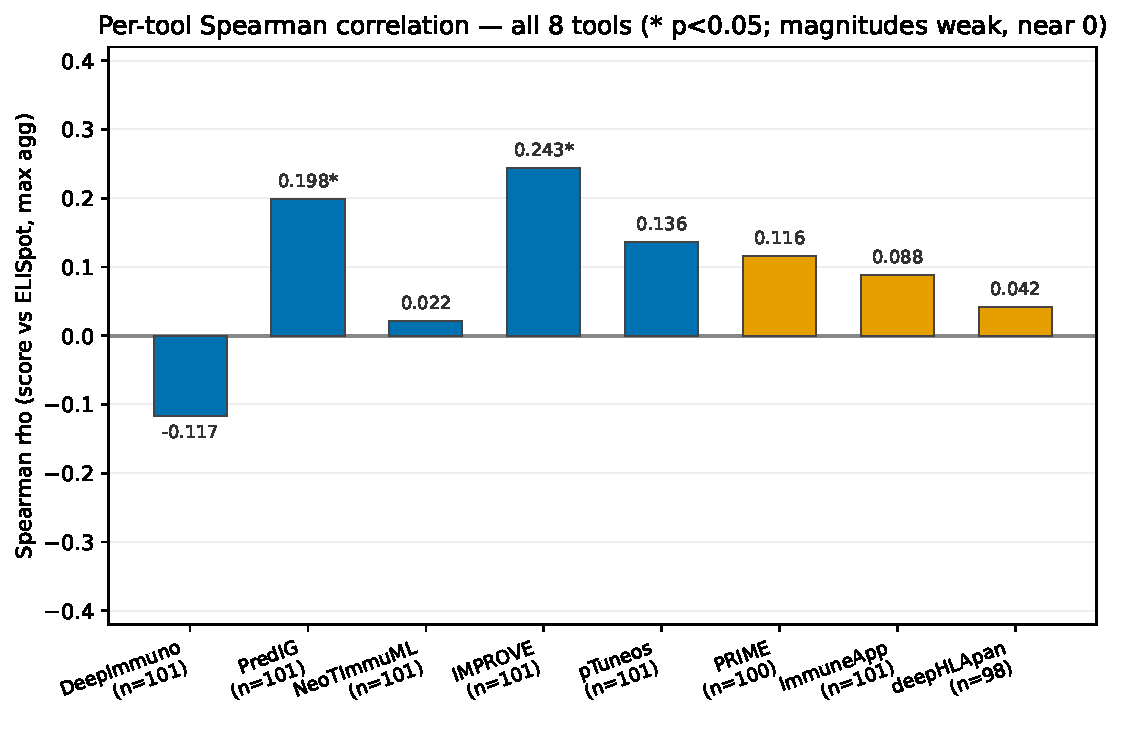
\includegraphics[width=\linewidth]{figures/fig7_spearman.pdf}
\caption{Spearman correlation between tool score and ELISpot SFC under
best-binder aggregation; $^{*}$ marks $p < 0.05$. All point estimates satisfy
$|\rho| < 0.33$.}
\label{fig:spearman}
\end{figure}

\subsection{Aggregation, threshold sensitivity, and bootstrap uncertainty}
\label{sec:res-sensitivity}

The point-estimate ordering in Table~\ref{tab:main} is fragile in two distinct
ways, and we report both so that the leading position is not mistaken for a
statistically established advantage.

\paragraph{Sensitivity to aggregation and threshold.} The leading AUC is not
stable across operating points. pTuneos rises to AUC $= 0.7813$ under mean
aggregation at the SFC $>0$ threshold, but the same tool falls to
$\approx 0.46$---below chance---when the threshold is moved to the cohort median,
indicating that its apparent discrimination is concentrated at one operating
point rather than reflecting a robust capability. Aggregation choice alone can
move a tool materially: ImmuneApp improves from AUC $= 0.5889$ under maximum
aggregation to $0.6444$ under mean aggregation at the same SFC $>0$ threshold
(a shift of $+0.055$), confirming that its score is sensitive to how the
per-window, per-allele values are summarized. These observations are exactly why
the headline comparison is locked to a single aggregation--threshold combination
(Section~\ref{sec:fairness}); allowing each tool its own best-of-nine operating
point (\emph{selection-on-max}) would award different tools different conventions
and is reported only descriptively. Under such per-tool best-of-nine selection,
the highest \emph{significant} magnitude correlations belong to IMPROVE
(top3mean aggregation, $\rho = 0.3202$, $p = 0.0011$) and PredIG (mean
aggregation, $\rho = 0.2797$, $p = 0.0046$); we present these as descriptive
upper envelopes per tool and not as a cross-tool ranking, since the operating
points differ.

\paragraph{Bootstrap uncertainty.} A $2000$-replicate bootstrap shows that the
leading AUC carries a wide confidence interval: pTuneos has AUC $= 0.7525$ with a
$95\%$ CI of $[0.598, 0.888]$. The per-tool intervals are wide and broadly
overlapping---for example PredIG $[0.490, 0.815]$ and NeoTImmuML$^\star$
$[0.498, 0.792]$ both overlap the pTuneos interval substantially. A paired
bootstrap of the between-tool AUC differences confirms that pTuneos's lead over
its nearest competitors is not significant: $\Delta\mathrm{AUC}$ against PredIG is
$0.0914$ with a $95\%$ CI of $[-0.145, 0.310]$, and against ImmuneApp is $0.1636$
with a CI of $[-0.093, 0.414]$, both spanning zero. We therefore describe pTuneos
as ranking first by point estimate, and we explicitly do not claim a single best
or strongest tool at the top of the panel. The same paired bootstrap does,
however, separate the upper group from the lower half: pTuneos's advantage reaches
significance against IMPROVE ($\Delta\mathrm{AUC} = 0.1318$, CI $[0.006, 0.287]$),
PRIME ($0.2283$, CI $[0.044, 0.434]$), and deepHLApan ($0.3517$, CI
$[0.040, 0.589]$), whose intervals exclude zero. This pattern is consistent with a
weak but real separation between an upper and a lower group of tools rather than a
single dominant predictor. The driver of the residual uncertainty is the cohort
size: DS2 contains $101$ peptides with only $11$ negatives, which is too small to
resolve AUC differences of the magnitude seen at the top of the table.

\begin{table}[t]
\centering
\caption{Bootstrap uncertainty on AUC-ROC under the locked configuration
($2000$ replicates). The leading tool's confidence interval is wide, and the
paired $\Delta\mathrm{AUC}$ intervals against its two nearest competitors
include zero (top block), so we do not claim a single best tool. The same paired
bootstrap does separate pTuneos from the lower half of the panel (bottom block),
whose intervals exclude zero.}
\label{tab:bootstrap}
\begin{tabular}{lcc}
\toprule
Comparison & $\Delta\mathrm{AUC}$ (point) & $95\%$ CI \\
\midrule
pTuneos AUC (absolute)                & $0.7525$ & $[0.598, 0.888]$ \\
\midrule
pTuneos $-$ PredIG                    & $0.0914$ & $[-0.145, 0.310]$ \\
pTuneos $-$ ImmuneApp                 & $0.1636$ & $[-0.093, 0.414]$ \\
\midrule
pTuneos $-$ IMPROVE                   & $0.1318$ & $[0.006, 0.287]$ \\
pTuneos $-$ PRIME                     & $0.2283$ & $[0.044, 0.434]$ \\
pTuneos $-$ deepHLApan                & $0.3517$ & $[0.040, 0.589]$ \\
\bottomrule
\end{tabular}

\vspace{2pt}
{\footnotesize A paired comparison against NeoTImmuML$^\star$ was not computed;
its overlapping per-tool interval ($[0.498, 0.792]$) is reported in the text.}
\end{table}

\begin{figure}[t]
\centering
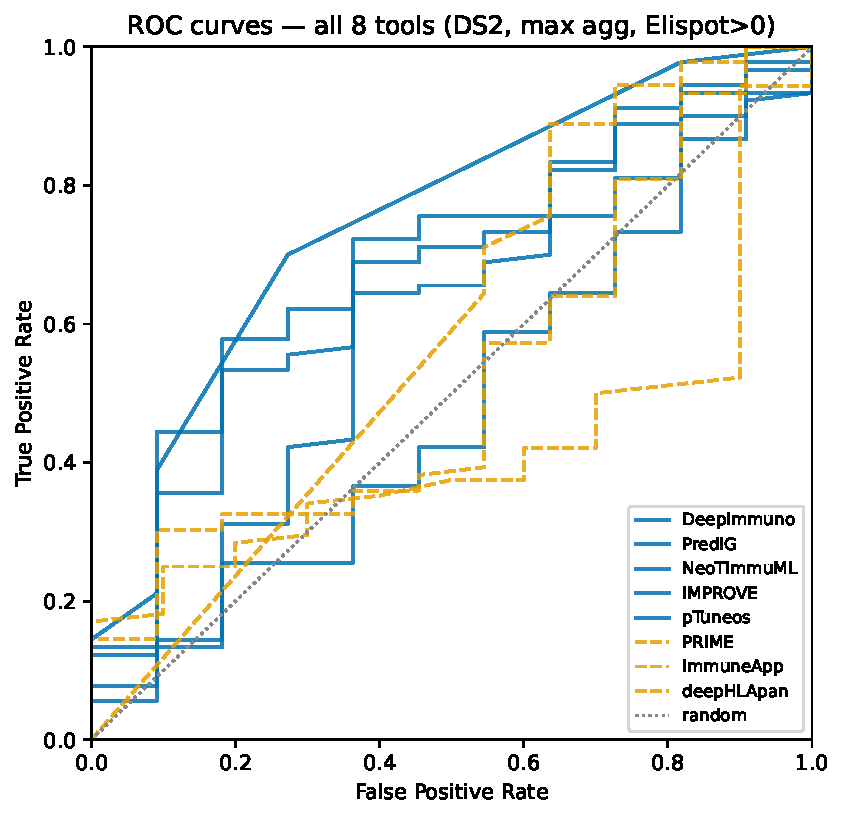
\includegraphics[width=\linewidth]{figures/fig8_roc_curves.pdf}
\caption{ROC curves for the eight tools at the SFC $>0$ threshold under
best-binder aggregation. New-wave tools are shown with dashed lines.}
\label{fig:roc}
\end{figure}

\subsection{Per-patient evaluation reorders the panel}
\label{sec:res-perpatient}

The global correlations in Table~\ref{tab:main} pool all peptides across patients
and can mask a tool's ability to rank candidates \emph{within} an individual
patient. Recomputing the magnitude correlation under the per-patient protocol of
Section~\ref{sec:perpatient}---a Fisher-$z$ weighted mean of the per-patient
$\rho_i$, with the median reported as a robust co-primary estimate---changes both
the magnitude and the ordering of the results (Table~\ref{tab:perpatient}).

% XXX_HLA-FIX[投稿前必更新]: 以下 per-patient 头条数字(PRIME 0.253/0.386, deepHLApan 0.261/0.402 等)均在含 P101/P102 等位伪迹的 9 患者上计算，修复后必变、相对排序可能动。待 Phase B 正确等位重推理后用 corrected 数据重算。数字暂不动=拍板点(P102 等位待袁老师确认)，见文件头 TODO + 04_LOG Entry HLA-FIX。
The most striking shifts occur for tools that are near the noise floor globally.
PRIME moves from a global $\rho = 0.1163$ to a per-patient Fisher-$z$ weighted
estimate of $0.253$ and a median of $0.386$, a change of $+0.270$ in the median
relative to the global value. Crucially, this jump is not an artifact of peptide
length: under best-binder aggregation PRIME's pooled peptide-level scores are
essentially uncorrelated with the number of constituent sub-peptides
($\rho \approx 0.13$), so the per-patient gain reflects a genuine within-patient
reordering rather than a length proxy. IMPROVE shows the same clean pattern, moving
from a global $\rho = 0.2434$ to a Fisher-$z$ estimate of $0.250$ and a median of
$0.268$, and its scores are likewise length-insensitive ($\rho \approx 0.12$).
DeepImmuno, which carries a negative global point estimate ($-0.1168$), moves to a
Fisher-$z$ estimate of $0.0127$ and a median of $-0.05$, i.e.\ toward zero but
without a meaningful within-patient signal. This
reordering shows that the global Spearman is not merely a noisy version of the
per-patient estimate; for some tools it has the wrong sign or magnitude because
it conflates between-patient and within-patient variation.

A large per-patient jump must not, however, be read uncritically as within-patient
capability, because the underlying peptide-level scores can themselves be
confounded. deepHLApan is the cautionary case. Its global $\rho = 0.0415$ rises to
a per-patient Fisher-$z$ estimate of $0.261$ and a median of $0.402$---numerically
the largest shift in the panel---but under best-binder aggregation its pooled
scores are strongly correlated with peptide length, as captured by the number of
constituent sub-peptides ($\rho \approx 0.57$), well above the $\rho = 0.5$ level
at which we treat an aggregation as count-confounded. Re-pooling deepHLApan with
length-insensitive operators---\texttt{mean} or the geometric mean, whose own
correlation with peptide length is negligible ($\rho \approx 0.08$)---collapses its
correlation with immunogenicity to $\approx 0$. The per-patient jump for deepHLApan
therefore largely tracks peptide length rather than within-patient immunogenicity
ranking, and we report it as a cautionary example---per-patient correlation does
not by itself remove aggregation-level confounds
(Section~\ref{sec:harmonization})---rather than as evidence of ranking ability.

Underneath these aggregates is substantial individual heterogeneity that the
global number averages away. The core methodological finding is that pooling can
cancel a genuine within-patient signal: PRIME's clean $+0.270$ median jump shows
that a tool dismissed as near-noise globally can in fact order candidates within
individual patients, a structure the cohort-wide Spearman conceals. The underlying
per-patient coefficients are also widely dispersed; for deepHLApan they range from
$-0.43$ to $+0.81$ with a standard deviation of $0.46$, so the tool appears to rank
candidates well within some patients and inversely within others. As noted above,
however, deepHLApan's positive tail is inflated by the peptide-length confound, so
we read this spread as descriptive only. This dispersion also bounds how strongly
we can state any per-patient claim. With only $K = 9$ patients and small
per-patient sample sizes ($n_i = 5$--$16$), the per-patient aggregates carry wide
confidence intervals; we therefore anchor the claim on the Fisher-$z$ weighted mean
and the median together, treat the dispersion as descriptive, and flag the
small-sample caveat explicitly rather than ranking tools by these estimates.

\begin{table}[t]
\centering
\caption{Global versus per-patient magnitude correlation under best-binder
aggregation. Per-patient estimates aggregate the within-patient $\rho_i$ over
$K = 9$ patients ($n_i = 5$--$16$); the Fisher-$z$ weighted mean and the median
are co-primary. $\Delta$ is the median minus the global value. The reordering is
largest for tools near the global noise floor; PRIME is a clean exemplar, whereas
deepHLApan ($^{\dagger}$) is count-confounded under best-binder aggregation (see
note). Estimates carry wide confidence intervals owing to small $K$ and $n_i$ and
are not used to rank tools.}
\label{tab:perpatient}
\begin{tabular}{lcccc}
\toprule
Tool & Global $\rho$ & Fisher-$z$ mean & Median $\tilde{\rho}$ & $\Delta$ (med.\ $-$ glob.) \\
\midrule
PRIME                  & $0.1163$  & $0.253$  & $0.386$  & $+0.270$ \\
deepHLApan$^{\dagger}$ & $0.0415$  & $0.261$  & $0.402$  & $+0.360$ \\
DeepImmuno             & $-0.1168$ & $0.0127$ & $-0.05$  & $+0.067$ \\
\bottomrule
\end{tabular}

\vspace{2pt}
{\footnotesize $^{\dagger}$deepHLApan's per-patient jump is count-confounded under
best-binder aggregation: its pooled scores correlate with peptide length
($\rho \approx 0.57$) and the signal collapses to $\approx 0$ under
length-insensitive pooling, so this row is a cautionary case rather than evidence
of within-patient ranking ability. Per-patient aggregates (Fisher-$z$ weighted
mean; median) for the remaining tools: IMPROVE $0.250$; $0.268$, PredIG $0.230$;
$0.291$, pTuneos $0.170$; $0.159$, NeoTImmuML$^\star$ $0.033$; $0.058$, ImmuneApp
$0.173$; $0.187$. IMPROVE and PredIG remain among the top of the panel under both
the global and the per-patient view.}
\end{table}

\begin{figure}[t]
\centering
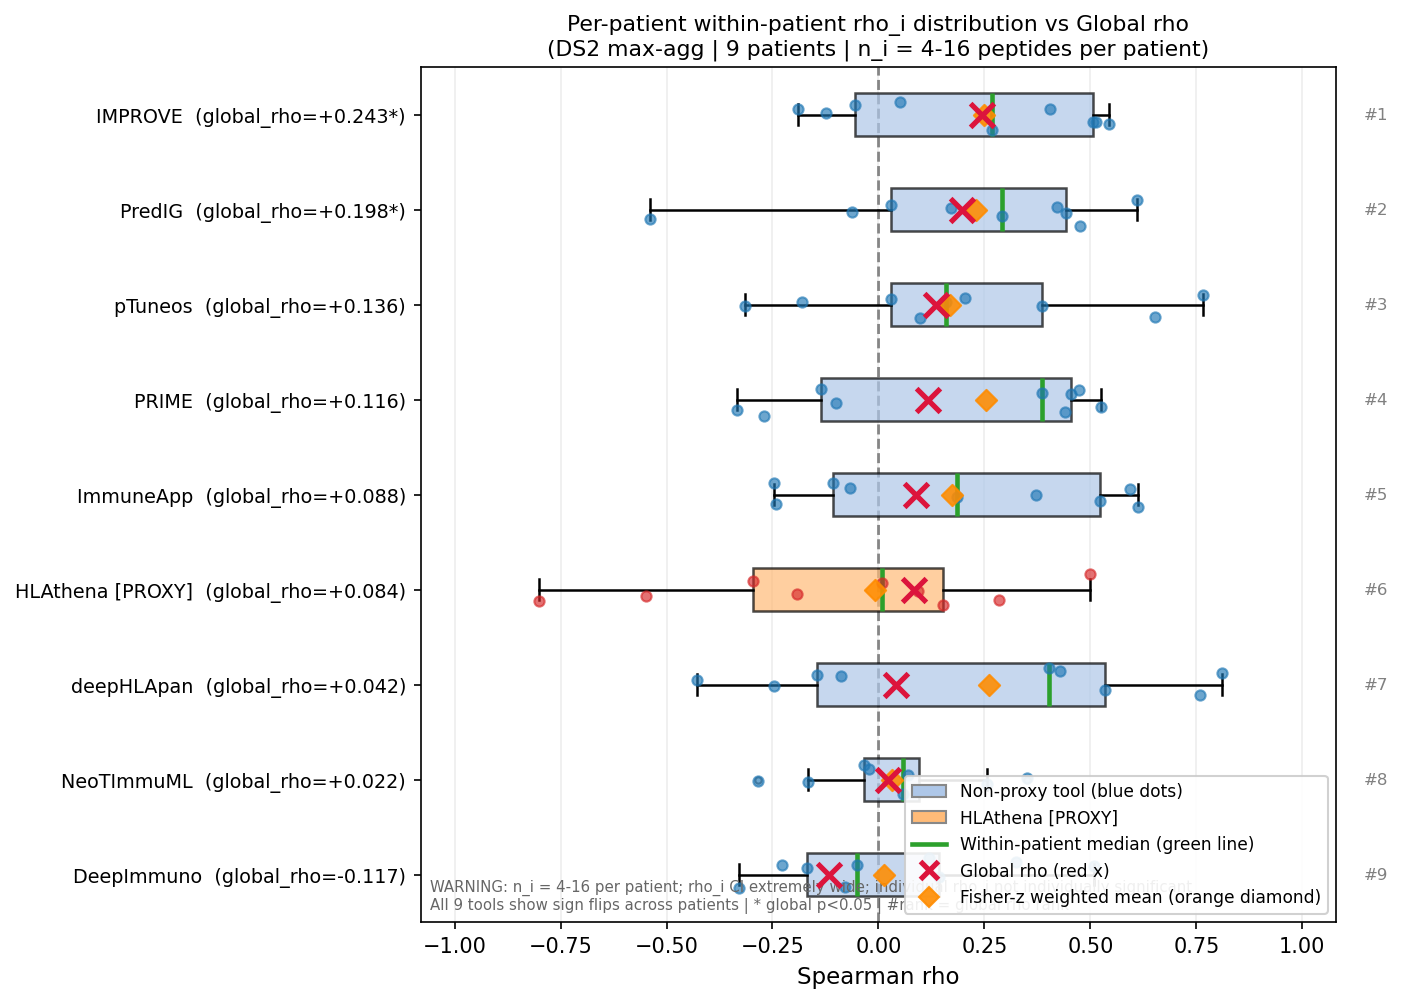
\includegraphics[width=\linewidth]{figures/fig9_perpatient.png}
% NOTE(coder): a dedicated per-patient rho_i strip/box plot with global vs Fisher-z/median
% overlay would sharpen this panel; current figure is the per-patient factor plot.
\caption{Distribution of per-patient $\rho_i$ for each tool, with the global
correlation and the Fisher-$z$/median aggregates overlaid. PRIME is a clean
exemplar of the heterogeneity hidden by the pooled estimate: a near-noise global
correlation ($\rho = 0.1163$) resolves into a positive within-patient median
($0.386$) with no peptide-length confound. The very wide spread for deepHLApan
($\rho_i \in [-0.43, +0.81]$, $\mathrm{std} = 0.46$) is shown for contrast, but
part of its positive tail reflects the peptide-length confound discussed in the
text and should not be read as within-patient ranking ability.}
\label{fig:perpatient}
\end{figure}

\subsection{Presentation proxy as a near-random anchor}
\label{sec:res-proxy}

Finally, the presentation proxy behaves as expected for a quantity that captures
peptide display rather than functional immunogenicity. HLAthena attains an
AUC of $\approx 0.51$ on the binary discrimination task---essentially random---and
its per-patient magnitude correlation is $\approx 0$. Because HLAthena scores
binding/presentation rather than T-cell activation, this near-random result is not
a failure of the proxy but a calibration anchor: it empirically separates the
three quantities at issue in this benchmark, namely presentation, immunogenicity
(positive/negative recognition), and magnitude (response strength). Presentation
is a necessary precondition for recognition, but on this cohort it carries no
information about either the binary recognition call or the continuous magnitude,
which is consistent with treating magnitude prediction as a distinct and
currently unmet capability (Section~\ref{sec:discussion}).
